\documentclass[1p]{elsarticle_modified}
%\bibliographystyle{elsarticle-num}

%\usepackage[colorlinks]{hyperref}
%\usepackage{abbrmath_seonhwa} %\Abb, \Ascr, \Acal ,\Abf, \Afrak
\usepackage{amsfonts}
\usepackage{amssymb}
\usepackage{amsmath}
\usepackage{amsthm}
\usepackage{scalefnt}
\usepackage{amsbsy}
\usepackage{kotex}
\usepackage{caption}
\usepackage{subfig}
\usepackage{color}
\usepackage{graphicx}
\usepackage{xcolor} %% white, black, red, green, blue, cyan, magenta, yellow
\usepackage{float}
\usepackage{setspace}
\usepackage{hyperref}

\usepackage{tikz}
\usetikzlibrary{arrows}

\usepackage{multirow}
\usepackage{array} % fixed length table
\usepackage{hhline}

%%%%%%%%%%%%%%%%%%%%%
\makeatletter
\renewcommand*\env@matrix[1][\arraystretch]{%
	\edef\arraystretch{#1}%
	\hskip -\arraycolsep
	\let\@ifnextchar\new@ifnextchar
	\array{*\c@MaxMatrixCols c}}
\makeatother %https://tex.stackexchange.com/questions/14071/how-can-i-increase-the-line-spacing-in-a-matrix
%%%%%%%%%%%%%%%

\usepackage[normalem]{ulem}

\newcommand{\msout}[1]{\ifmmode\text{\sout{\ensuremath{#1}}}\else\sout{#1}\fi}
%SOURCE: \msout is \stkout macro in https://tex.stackexchange.com/questions/20609/strikeout-in-math-mode

\newcommand{\cancel}[1]{
	\ifmmode
	{\color{red}\msout{#1}}
	\else
	{\color{red}\sout{#1}}
	\fi
}

\newcommand{\add}[1]{
	{\color{blue}\uwave{#1}}
}

\newcommand{\replace}[2]{
	\ifmmode
	{\color{red}\msout{#1}}{\color{blue}\uwave{#2}}
	\else
	{\color{red}\sout{#1}}{\color{blue}\uwave{#2}}
	\fi
}

\newcommand{\Sol}{\mathcal{S}} %segment
\newcommand{\D}{D} %diagram
\newcommand{\A}{\mathcal{A}} %arc


%%%%%%%%%%%%%%%%%%%%%%%%%%%%%5 test

\def\sl{\operatorname{\textup{SL}}(2,\Cbb)}
\def\psl{\operatorname{\textup{PSL}}(2,\Cbb)}
\def\quan{\mkern 1mu \triangleright \mkern 1mu}

\theoremstyle{definition}
\newtheorem{thm}{Theorem}[section]
\newtheorem{prop}[thm]{Proposition}
\newtheorem{lem}[thm]{Lemma}
\newtheorem{ques}[thm]{Question}
\newtheorem{cor}[thm]{Corollary}
\newtheorem{defn}[thm]{Definition}
\newtheorem{exam}[thm]{Example}
\newtheorem{rmk}[thm]{Remark}
\newtheorem{alg}[thm]{Algorithm}

\newcommand{\I}{\sqrt{-1}}
\begin{document}

%\begin{frontmatter}
%
%\title{Boundary parabolic representations of knots up to 8 crossings}
%
%%% Group authors per affiliation:
%\author{Yunhi Cho} 
%\address{Department of Mathematics, University of Seoul, Seoul, Korea}
%\ead{yhcho@uos.ac.kr}
%
%
%\author{Seonhwa Kim} %\fnref{s_kim}}
%\address{Center for Geometry and Physics, Institute for Basic Science, Pohang, 37673, Korea}
%\ead{ryeona17@ibs.re.kr}
%
%\author{Hyuk Kim}
%\address{Department of Mathematical Sciences, Seoul National University, Seoul 08826, Korea}
%\ead{hyukkim@snu.ac.kr}
%
%\author{Seokbeom Yoon}
%\address{Department of Mathematical Sciences, Seoul National University, Seoul, 08826,  Korea}
%\ead{sbyoon15@snu.ac.kr}
%
%\begin{abstract}
%We find all boundary parabolic representation of knots up to 8 crossings.
%
%\end{abstract}
%\begin{keyword}
%    \MSC[2010] 57M25 
%\end{keyword}
%
%\end{frontmatter}

%\linenumbers
%\tableofcontents
%
\newcommand\colored[1]{\textcolor{white}{\rule[-0.35ex]{0.8em}{1.4ex}}\kern-0.8em\color{red} #1}%
%\newcommand\colored[1]{\textcolor{white}{ #1}\kern-2.17ex	\textcolor{white}{ #1}\kern-1.81ex	\textcolor{white}{ #1}\kern-2.15ex\color{red}#1	}

{\Large $\underline{12n_{0439}~(K12n_{0439})}$}

\setlength{\tabcolsep}{10pt}
\renewcommand{\arraystretch}{1.6}
\vspace{1cm}\begin{tabular}{m{100pt}>{\centering\arraybackslash}m{274pt}}
\multirow{5}{120pt}{
	\centering
	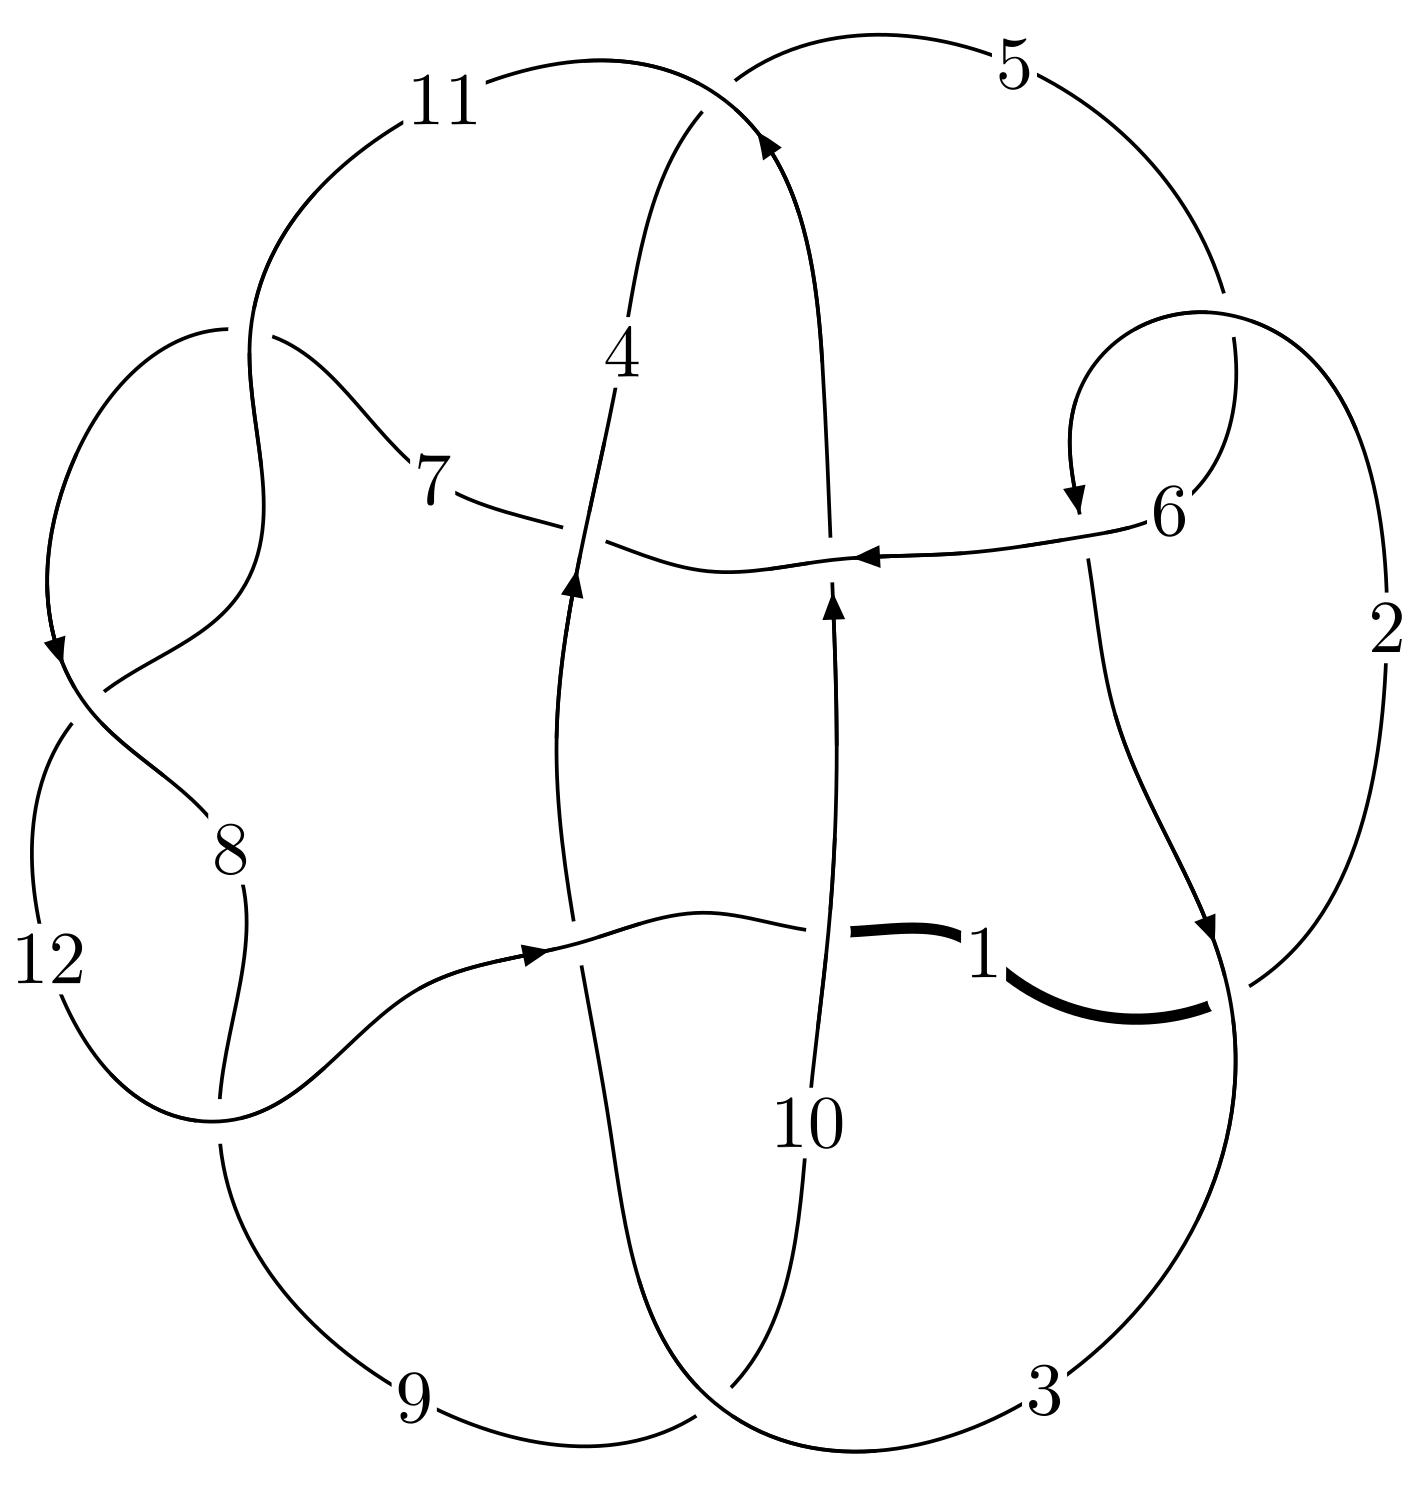
\includegraphics[width=112pt]{../../../GIT/diagram.site/Diagrams/png/2528_12n_0439.png}\\
\ \ \ A knot diagram\footnotemark}&
\allowdisplaybreaks
\textbf{Linearized knot diagam} \\
\cline{2-2}
 &
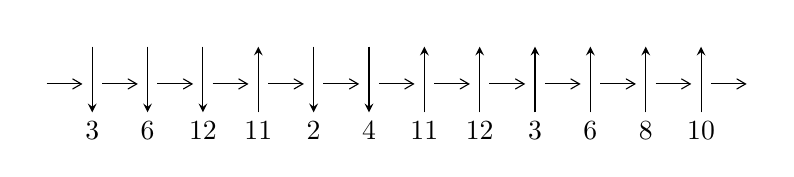
\begin{tikzpicture}[x=20pt, y=17pt]
	% nodes
	\node (C0) at (0, 0) {};
	\node (C1) at (1, 0) {};
	\node (C1U) at (1, +1) {};
	\node (C1D) at (1, -1) {3};

	\node (C2) at (2, 0) {};
	\node (C2U) at (2, +1) {};
	\node (C2D) at (2, -1) {6};

	\node (C3) at (3, 0) {};
	\node (C3U) at (3, +1) {};
	\node (C3D) at (3, -1) {12};

	\node (C4) at (4, 0) {};
	\node (C4U) at (4, +1) {};
	\node (C4D) at (4, -1) {11};

	\node (C5) at (5, 0) {};
	\node (C5U) at (5, +1) {};
	\node (C5D) at (5, -1) {2};

	\node (C6) at (6, 0) {};
	\node (C6U) at (6, +1) {};
	\node (C6D) at (6, -1) {4};

	\node (C7) at (7, 0) {};
	\node (C7U) at (7, +1) {};
	\node (C7D) at (7, -1) {11};

	\node (C8) at (8, 0) {};
	\node (C8U) at (8, +1) {};
	\node (C8D) at (8, -1) {12};

	\node (C9) at (9, 0) {};
	\node (C9U) at (9, +1) {};
	\node (C9D) at (9, -1) {3};

	\node (C10) at (10, 0) {};
	\node (C10U) at (10, +1) {};
	\node (C10D) at (10, -1) {6};

	\node (C11) at (11, 0) {};
	\node (C11U) at (11, +1) {};
	\node (C11D) at (11, -1) {8};

	\node (C12) at (12, 0) {};
	\node (C12U) at (12, +1) {};
	\node (C12D) at (12, -1) {10};
	\node (C13) at (13, 0) {};

	% arrows
	\draw[->,>={angle 60}]
	(C0) edge (C1) (C1) edge (C2) (C2) edge (C3) (C3) edge (C4) (C4) edge (C5) (C5) edge (C6) (C6) edge (C7) (C7) edge (C8) (C8) edge (C9) (C9) edge (C10) (C10) edge (C11) (C11) edge (C12) (C12) edge (C13) ;	\draw[->,>=stealth]
	(C1U) edge (C1D) (C2U) edge (C2D) (C3U) edge (C3D) (C4D) edge (C4U) (C5U) edge (C5D) (C6U) edge (C6D) (C7D) edge (C7U) (C8D) edge (C8U) (C9D) edge (C9U) (C10D) edge (C10U) (C11D) edge (C11U) (C12D) edge (C12U) ;
	\end{tikzpicture} \\
\hhline{~~} \\& 
\textbf{Solving Sequence} \\ \cline{2-2} 
 &
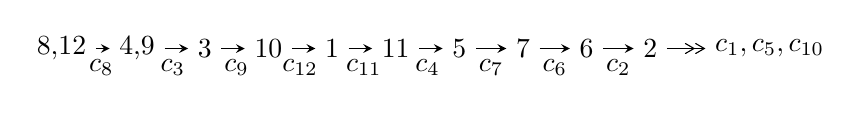
\begin{tikzpicture}[x=23pt, y=7pt]
	% node
	\node (A0) at (-1/8, 0) {8,12};
	\node (A1) at (17/16, 0) {4,9};
	\node (A2) at (17/8, 0) {3};
	\node (A3) at (25/8, 0) {10};
	\node (A4) at (33/8, 0) {1};
	\node (A5) at (41/8, 0) {11};
	\node (A6) at (49/8, 0) {5};
	\node (A7) at (57/8, 0) {7};
	\node (A8) at (65/8, 0) {6};
	\node (A9) at (73/8, 0) {2};
	\node (C1) at (1/2, -1) {$c_{8}$};
	\node (C2) at (13/8, -1) {$c_{3}$};
	\node (C3) at (21/8, -1) {$c_{9}$};
	\node (C4) at (29/8, -1) {$c_{12}$};
	\node (C5) at (37/8, -1) {$c_{11}$};
	\node (C6) at (45/8, -1) {$c_{4}$};
	\node (C7) at (53/8, -1) {$c_{7}$};
	\node (C8) at (61/8, -1) {$c_{6}$};
	\node (C9) at (69/8, -1) {$c_{2}$};
	\node (A10) at (11, 0) {$c_{1},c_{5},c_{10}$};

	% edge
	\draw[->,>=stealth]	
	(A0) edge (A1) (A1) edge (A2) (A2) edge (A3) (A3) edge (A4) (A4) edge (A5) (A5) edge (A6) (A6) edge (A7) (A7) edge (A8) (A8) edge (A9) ;
	\draw[->>,>={angle 60}]	
	(A9) edge (A10);
\end{tikzpicture} \\ 

\end{tabular} \\

\footnotetext{
The image of knot diagram is generated by the software ``\textbf{Draw programme}" developed by Andrew Bartholomew(\url{http://www.layer8.co.uk/maths/draw/index.htm\#Running-draw}), where we modified some parts for our purpose(\url{https://github.com/CATsTAILs/LinksPainter}).
}\phantom \\ \newline 
\centering \textbf{Ideals for irreducible components\footnotemark of $X_{\text{par}}$} 
 
\begin{align*}
I^u_{1}&=\langle 
-51 u^8+4 u^7+487 u^6+424 u^5-1094 u^4-281 u^3+1891 u^2+551 b+812 u+165,\\
\phantom{I^u_{1}}&\phantom{= \langle  }267 u^8+919 u^7+173 u^6-2317 u^5+185 u^4+5555 u^3+2060 u^2+1102 a-2436 u-799,\\
\phantom{I^u_{1}}&\phantom{= \langle  }u^9+5 u^8+7 u^7-3 u^6-7 u^5+17 u^4+32 u^3+18 u^2+7 u+2\rangle \\
I^u_{2}&=\langle 
u^7-2 u^6- u^5+5 u^4-2 u^3-5 u^2+b+2 u+2,\;- u^7+3 u^6- u^5-4 u^4+3 u^3+3 u^2+3 a- u-4,\\
\phantom{I^u_{2}}&\phantom{= \langle  }u^8-3 u^7+u^6+7 u^5-9 u^4-3 u^3+10 u^2-2 u-3\rangle \\
I^u_{3}&=\langle 
b+2 a-1,\;4 a^2-6 a+7,\;u-2\rangle \\
\\
I^v_{1}&=\langle 
a,\;b+v,\;v^2- v+1\rangle \\
\end{align*}
\raggedright * 4 irreducible components of $\dim_{\mathbb{C}}=0$, with total 21 representations.\\
\footnotetext{All coefficients of polynomials are rational numbers. But the coefficients are sometimes approximated in decimal forms when there is not enough margin.}
\newpage
\renewcommand{\arraystretch}{1}
\centering \section*{I. $I^u_{1}= \langle -51 u^8+4 u^7+\cdots+551 b+165,\;267 u^8+919 u^7+\cdots+1102 a-799,\;u^9+5 u^8+\cdots+7 u+2 \rangle$}
\flushleft \textbf{(i) Arc colorings}\\
\begin{tabular}{m{7pt} m{180pt} m{7pt} m{180pt} }
\flushright $a_{8}=$&$\begin{pmatrix}1\\0\end{pmatrix}$ \\
\flushright $a_{12}=$&$\begin{pmatrix}0\\u\end{pmatrix}$ \\
\flushright $a_{4}=$&$\begin{pmatrix}-0.242287 u^{8}-0.833938 u^{7}+\cdots+2.21053 u+0.725045\\0.0925590 u^{8}-0.00725953 u^{7}+\cdots-1.47368 u-0.299456\end{pmatrix}$ \\
\flushright $a_{9}=$&$\begin{pmatrix}1\\- u^2\end{pmatrix}$ \\
\flushright $a_{3}=$&$\begin{pmatrix}-0.242287 u^{8}-0.833938 u^{7}+\cdots+2.21053 u+0.725045\\0.441016 u^{8}+1.25953 u^{7}+\cdots+0.684211 u+0.455535\end{pmatrix}$ \\
\flushright $a_{10}=$&$\begin{pmatrix}0.0735027 u^{8}+0.376588 u^{7}+\cdots-0.0526316 u+0.409256\\-0.0326679 u^{8}-0.0562613 u^{7}+\cdots+0.578947 u-0.0707804\end{pmatrix}$ \\
\flushright $a_{1}=$&$\begin{pmatrix}-0.0408348 u^{8}-0.320327 u^{7}+\cdots-0.526316 u-0.338475\\-0.0907441 u^{8}+0.399274 u^{7}+\cdots+2.05263 u+0.470054\end{pmatrix}$ \\
\flushright $a_{11}=$&$\begin{pmatrix}- u\\u\end{pmatrix}$ \\
\flushright $a_{5}=$&$\begin{pmatrix}0.227768 u^{8}+0.697822 u^{7}+\cdots+3.15789 u+0.910163\\-0.377495 u^{8}-1.53902 u^{7}+\cdots-2.42105 u-0.484574\end{pmatrix}$ \\
\flushright $a_{7}=$&$\begin{pmatrix}- u^2+1\\u^2\end{pmatrix}$ \\
\flushright $a_{6}=$&$\begin{pmatrix}0.0825771 u^{8}+0.336661 u^{7}+\cdots-1.15789 u+0.262250\\-0.00907441 u^{8}+0.0399274 u^{7}+\cdots+1.10526 u+0.147005\end{pmatrix}$ \\
\flushright $a_{2}=$&$\begin{pmatrix}-0.0735027 u^{8}-0.376588 u^{7}+\cdots+1.05263 u+0.590744\\-0.0762250 u^{8}-0.464610 u^{7}+\cdots-0.315789 u-0.165154\end{pmatrix}$\\&\end{tabular}
\flushleft \textbf{(ii) Obstruction class $= -1$}\\~\\
\flushleft \textbf{(iii) Cusp Shapes $= \frac{1779}{551} u^8+\frac{8482}{551} u^7+\frac{9752}{551} u^6-\frac{10058}{551} u^5-\frac{11137}{551} u^4+\frac{36963}{551} u^3+\frac{46798}{551} u^2+\frac{379}{19} u+\frac{5232}{551}$}\\~\\
\newpage\renewcommand{\arraystretch}{1}
\flushleft \textbf{(iv) u-Polynomials at the component}\newline \\
\begin{tabular}{m{50pt}|m{274pt}}
Crossings & \hspace{64pt}u-Polynomials at each crossing \\
\hline $$\begin{aligned}c_{1}\end{aligned}$$&$\begin{aligned}
&u^9+6 u^8+\cdots+1105 u+16
\end{aligned}$\\
\hline $$\begin{aligned}c_{2},c_{5}\end{aligned}$$&$\begin{aligned}
&u^9+6 u^8+15 u^7+19 u^6+39 u^5+96 u^4+137 u^3+93 u^2+19 u-4
\end{aligned}$\\
\hline $$\begin{aligned}c_{3},c_{6}\end{aligned}$$&$\begin{aligned}
&u^9- u^8+6 u^7+6 u^6+39 u^5+60 u^4+40 u^3+13 u^2+u-1
\end{aligned}$\\
\hline $$\begin{aligned}c_{4},c_{9}\end{aligned}$$&$\begin{aligned}
&u^9+u^8+7 u^7+9 u^6+14 u^5+11 u^4+8 u^3+u^2- u-1
\end{aligned}$\\
\hline $$\begin{aligned}c_{7},c_{8},c_{11}\end{aligned}$$&$\begin{aligned}
&u^9-5 u^8+7 u^7+3 u^6-7 u^5-17 u^4+32 u^3-18 u^2+7 u-2
\end{aligned}$\\
\hline $$\begin{aligned}c_{10},c_{12}\end{aligned}$$&$\begin{aligned}
&u^9+6 u^8+14 u^7-5 u^6+66 u^5-202 u^4+132 u^3+u^2-10 u-1
\end{aligned}$\\
\hline
\end{tabular}\\~\\
\newpage\renewcommand{\arraystretch}{1}
\flushleft \textbf{(v) Riley Polynomials at the component}\newline \\
\begin{tabular}{m{50pt}|m{274pt}}
Crossings & \hspace{64pt}Riley Polynomials at each crossing \\
\hline $$\begin{aligned}c_{1}\end{aligned}$$&$\begin{aligned}
&y^9+114 y^8+\cdots+1135425 y-256
\end{aligned}$\\
\hline $$\begin{aligned}c_{2},c_{5}\end{aligned}$$&$\begin{aligned}
&y^9-6 y^8+\cdots+1105 y-16
\end{aligned}$\\
\hline $$\begin{aligned}c_{3},c_{6}\end{aligned}$$&$\begin{aligned}
&y^9+11 y^8+\cdots+27 y-1
\end{aligned}$\\
\hline $$\begin{aligned}c_{4},c_{9}\end{aligned}$$&$\begin{aligned}
&y^9+13 y^8+59 y^7+109 y^6+106 y^5+73 y^4+32 y^3+5 y^2+3 y-1
\end{aligned}$\\
\hline $$\begin{aligned}c_{7},c_{8},c_{11}\end{aligned}$$&$\begin{aligned}
&y^9-11 y^8+\cdots-23 y-4
\end{aligned}$\\
\hline $$\begin{aligned}c_{10},c_{12}\end{aligned}$$&$\begin{aligned}
&y^9-8 y^8+\cdots+102 y-1
\end{aligned}$\\
\hline
\end{tabular}\\~\\
\newpage\flushleft \textbf{(vi) Complex Volumes and Cusp Shapes}
$$\begin{array}{c|c|c}  
\text{Solutions to }I^u_{1}& \I (\text{vol} + \sqrt{-1}CS) & \text{Cusp shape}\\
 \hline 
\begin{aligned}
u &= \phantom{-}1.18169 + 0.81660 I \\
a &= -1.13356 - 0.92427 I \\
b &= \phantom{-}0.538744 + 0.723261 I\end{aligned}
 & \phantom{-}4.72372 - 1.44557 I & \phantom{-}2.79413 + 0.05589 I \\ \hline\begin{aligned}
u &= \phantom{-}1.18169 - 0.81660 I \\
a &= -1.13356 + 0.92427 I \\
b &= \phantom{-}0.538744 - 0.723261 I\end{aligned}
 & \phantom{-}4.72372 + 1.44557 I & \phantom{-}2.79413 - 0.05589 I \\ \hline\begin{aligned}
u &= -0.557684\phantom{ +0.000000I} \\
a &= -0.337455\phantom{ +0.000000I} \\
b &= -0.425472\phantom{ +0.000000I}\end{aligned}
 & \phantom{-}0.803810\phantom{ +0.000000I} & \phantom{-}12.4850\phantom{ +0.000000I} \\ \hline\begin{aligned}
u &= -1.42962 + 0.20941 I \\
a &= \phantom{-}0.119321 + 0.349200 I \\
b &= -0.023607 - 1.115360 I\end{aligned}
 & \phantom{-}3.18435 - 3.04209 I & \phantom{-}1.27965 + 3.40109 I \\ \hline\begin{aligned}
u &= -1.42962 - 0.20941 I \\
a &= \phantom{-}0.119321 - 0.349200 I \\
b &= -0.023607 + 1.115360 I\end{aligned}
 & \phantom{-}3.18435 + 3.04209 I & \phantom{-}1.27965 - 3.40109 I \\ \hline\begin{aligned}
u &= -0.058623 + 0.424215 I \\
a &= \phantom{-}0.74163 + 1.41569 I \\
b &= \phantom{-}0.476502 - 0.460767 I\end{aligned}
 & -1.48784 + 0.34537 I & -5.00907 - 1.24859 I \\ \hline\begin{aligned}
u &= -0.058623 - 0.424215 I \\
a &= \phantom{-}0.74163 - 1.41569 I \\
b &= \phantom{-}0.476502 + 0.460767 I\end{aligned}
 & -1.48784 - 0.34537 I & -5.00907 + 1.24859 I \\ \hline\begin{aligned}
u &= -1.91461 + 0.93499 I \\
a &= -0.308657 - 1.376960 I \\
b &= -0.27890 + 2.28182 I\end{aligned}
 & \phantom{-}13.7395 - 8.2460 I & \phantom{-}2.69287 + 2.56767 I \\ \hline\begin{aligned}
u &= -1.91461 - 0.93499 I \\
a &= -0.308657 + 1.376960 I \\
b &= -0.27890 - 2.28182 I\end{aligned}
 & \phantom{-}13.7395 + 8.2460 I & \phantom{-}2.69287 - 2.56767 I\\
 \hline 
 \end{array}$$\newpage\newpage\renewcommand{\arraystretch}{1}
\centering \section*{II. $I^u_{2}= \langle u^7-2 u^6- u^5+5 u^4-2 u^3-5 u^2+b+2 u+2,\;- u^7+3 u^6+\cdots+3 a-4,\;u^8-3 u^7+\cdots-2 u-3 \rangle$}
\flushleft \textbf{(i) Arc colorings}\\
\begin{tabular}{m{7pt} m{180pt} m{7pt} m{180pt} }
\flushright $a_{8}=$&$\begin{pmatrix}1\\0\end{pmatrix}$ \\
\flushright $a_{12}=$&$\begin{pmatrix}0\\u\end{pmatrix}$ \\
\flushright $a_{4}=$&$\begin{pmatrix}\frac{1}{3} u^7- u^6+\cdots+\frac{1}{3} u+\frac{4}{3}\\- u^7+2 u^6+u^5-5 u^4+2 u^3+5 u^2-2 u-2\end{pmatrix}$ \\
\flushright $a_{9}=$&$\begin{pmatrix}1\\- u^2\end{pmatrix}$ \\
\flushright $a_{3}=$&$\begin{pmatrix}\frac{1}{3} u^7- u^6+\cdots+\frac{1}{3} u+\frac{4}{3}\\- u^7+3 u^6- u^5-5 u^4+5 u^3+3 u^2-3 u-2\end{pmatrix}$ \\
\flushright $a_{10}=$&$\begin{pmatrix}\frac{2}{3} u^7- u^6+\cdots+\frac{2}{3} u+\frac{8}{3}\\- u^7+u^6+2 u^5-4 u^4- u^3+5 u^2+u-1\end{pmatrix}$ \\
\flushright $a_{1}=$&$\begin{pmatrix}\frac{1}{3} u^7-\frac{2}{3} u^5+\cdots-\frac{5}{3} u-\frac{5}{3}\\2 u^7-5 u^6-2 u^5+14 u^4-8 u^3-15 u^2+11 u+7\end{pmatrix}$ \\
\flushright $a_{11}=$&$\begin{pmatrix}- u\\u\end{pmatrix}$ \\
\flushright $a_{5}=$&$\begin{pmatrix}-\frac{2}{3} u^7+u^6+\cdots-\frac{11}{3} u-\frac{5}{3}\\- u^5+2 u^4-3 u^2+2 u+1\end{pmatrix}$ \\
\flushright $a_{7}=$&$\begin{pmatrix}- u^2+1\\u^2\end{pmatrix}$ \\
\flushright $a_{6}=$&$\begin{pmatrix}-\frac{1}{3} u^7+u^6+\cdots-\frac{7}{3} u+\frac{2}{3}\\u^7-2 u^6- u^5+6 u^4-3 u^3-5 u^2+3 u+2\end{pmatrix}$ \\
\flushright $a_{2}=$&$\begin{pmatrix}\frac{2}{3} u^7- u^6+\cdots+\frac{5}{3} u+\frac{5}{3}\\- u^3+u^2-1\end{pmatrix}$\\&\end{tabular}
\flushleft \textbf{(ii) Obstruction class $= 1$}\\~\\
\flushleft \textbf{(iii) Cusp Shapes $= 3 u^7-7 u^6+3 u^5+10 u^4-12 u^3-2 u^2+3 u+3$}\\~\\
\newpage\renewcommand{\arraystretch}{1}
\flushleft \textbf{(iv) u-Polynomials at the component}\newline \\
\begin{tabular}{m{50pt}|m{274pt}}
Crossings & \hspace{64pt}u-Polynomials at each crossing \\
\hline $$\begin{aligned}c_{1}\end{aligned}$$&$\begin{aligned}
&u^8-10 u^7+39 u^6-81 u^5+117 u^4-122 u^3+63 u^2-11 u+1
\end{aligned}$\\
\hline $$\begin{aligned}c_{2}\end{aligned}$$&$\begin{aligned}
&u^8+4 u^7+3 u^6-7 u^5-13 u^4-4 u^3+7 u^2+5 u+1
\end{aligned}$\\
\hline $$\begin{aligned}c_{3},c_{6}\end{aligned}$$&$\begin{aligned}
&u^8+2 u^7-2 u^5-3 u^4-3 u^3+3 u^2+4 u+1
\end{aligned}$\\
\hline $$\begin{aligned}c_{4},c_{9}\end{aligned}$$&$\begin{aligned}
&u^8+7 u^6+10 u^4-5 u^3- u^2-2 u-1
\end{aligned}$\\
\hline $$\begin{aligned}c_{5}\end{aligned}$$&$\begin{aligned}
&u^8-4 u^7+3 u^6+7 u^5-13 u^4+4 u^3+7 u^2-5 u+1
\end{aligned}$\\
\hline $$\begin{aligned}c_{7},c_{8}\end{aligned}$$&$\begin{aligned}
&u^8-3 u^7+u^6+7 u^5-9 u^4-3 u^3+10 u^2-2 u-3
\end{aligned}$\\
\hline $$\begin{aligned}c_{10},c_{12}\end{aligned}$$&$\begin{aligned}
&u^8+u^7+3 u^6+2 u^5-6 u^4+6 u^3-8 u^2+5 u-1
\end{aligned}$\\
\hline $$\begin{aligned}c_{11}\end{aligned}$$&$\begin{aligned}
&u^8+3 u^7+u^6-7 u^5-9 u^4+3 u^3+10 u^2+2 u-3
\end{aligned}$\\
\hline
\end{tabular}\\~\\
\newpage\renewcommand{\arraystretch}{1}
\flushleft \textbf{(v) Riley Polynomials at the component}\newline \\
\begin{tabular}{m{50pt}|m{274pt}}
Crossings & \hspace{64pt}Riley Polynomials at each crossing \\
\hline $$\begin{aligned}c_{1}\end{aligned}$$&$\begin{aligned}
&y^8-22 y^7+135 y^6+251 y^5-1379 y^4-1846 y^3+1519 y^2+5 y+1
\end{aligned}$\\
\hline $$\begin{aligned}c_{2},c_{5}\end{aligned}$$&$\begin{aligned}
&y^8-10 y^7+39 y^6-81 y^5+117 y^4-122 y^3+63 y^2-11 y+1
\end{aligned}$\\
\hline $$\begin{aligned}c_{3},c_{6}\end{aligned}$$&$\begin{aligned}
&y^8-4 y^7+2 y^6+14 y^5-17 y^4-11 y^3+27 y^2-10 y+1
\end{aligned}$\\
\hline $$\begin{aligned}c_{4},c_{9}\end{aligned}$$&$\begin{aligned}
&y^8+14 y^7+69 y^6+138 y^5+84 y^4-59 y^3-39 y^2-2 y+1
\end{aligned}$\\
\hline $$\begin{aligned}c_{7},c_{8},c_{11}\end{aligned}$$&$\begin{aligned}
&y^8-7 y^7+25 y^6-65 y^5+125 y^4-167 y^3+142 y^2-64 y+9
\end{aligned}$\\
\hline $$\begin{aligned}c_{10},c_{12}\end{aligned}$$&$\begin{aligned}
&y^8+5 y^7-7 y^6-68 y^5-48 y^4+34 y^3+16 y^2-9 y+1
\end{aligned}$\\
\hline
\end{tabular}\\~\\
\newpage\flushleft \textbf{(vi) Complex Volumes and Cusp Shapes}
$$\begin{array}{c|c|c}  
\text{Solutions to }I^u_{2}& \I (\text{vol} + \sqrt{-1}CS) & \text{Cusp shape}\\
 \hline 
\begin{aligned}
u &= -1.143550 + 0.105994 I \\
a &= \phantom{-}0.027839 + 1.059490 I \\
b &= -0.039265 - 0.565787 I\end{aligned}
 & \phantom{-}4.97207 - 3.05412 I & \phantom{-}5.35335 + 5.43549 I \\ \hline\begin{aligned}
u &= -1.143550 - 0.105994 I \\
a &= \phantom{-}0.027839 - 1.059490 I \\
b &= -0.039265 + 0.565787 I\end{aligned}
 & \phantom{-}4.97207 + 3.05412 I & \phantom{-}5.35335 - 5.43549 I \\ \hline\begin{aligned}
u &= \phantom{-}1.084730 + 0.492548 I \\
a &= \phantom{-}0.753232 - 0.582528 I \\
b &= \phantom{-}0.13996 + 2.26543 I\end{aligned}
 & -12.04710 + 1.95234 I & -1.37368 - 3.45942 I \\ \hline\begin{aligned}
u &= \phantom{-}1.084730 - 0.492548 I \\
a &= \phantom{-}0.753232 + 0.582528 I \\
b &= \phantom{-}0.13996 - 2.26543 I\end{aligned}
 & -12.04710 - 1.95234 I & -1.37368 + 3.45942 I \\ \hline\begin{aligned}
u &= \phantom{-}1.03265 + 1.04538 I \\
a &= -0.527623 + 0.897663 I \\
b &= -0.31449 - 1.42869 I\end{aligned}
 & -5.86984 + 3.80835 I & \phantom{-}2.98023 - 3.30420 I \\ \hline\begin{aligned}
u &= \phantom{-}1.03265 - 1.04538 I \\
a &= -0.527623 - 0.897663 I \\
b &= -0.31449 + 1.42869 I\end{aligned}
 & -5.86984 - 3.80835 I & \phantom{-}2.98023 + 3.30420 I \\ \hline\begin{aligned}
u &= -0.483343\phantom{ +0.000000I} \\
a &= \phantom{-}1.10069\phantom{ +0.000000I} \\
b &= -0.358657\phantom{ +0.000000I}\end{aligned}
 & -0.371792\phantom{ +0.000000I} & \phantom{-}2.79670\phantom{ +0.000000I} \\ \hline\begin{aligned}
u &= \phantom{-}1.53567\phantom{ +0.000000I} \\
a &= -0.274253\phantom{ +0.000000I} \\
b &= \phantom{-}0.786231\phantom{ +0.000000I}\end{aligned}
 & \phantom{-}6.52231\phantom{ +0.000000I} & \phantom{-}9.28350\phantom{ +0.000000I}\\
 \hline 
 \end{array}$$\newpage\newpage\renewcommand{\arraystretch}{1}
\centering \section*{III. $I^u_{3}= \langle b+2 a-1,\;4 a^2-6 a+7,\;u-2 \rangle$}
\flushleft \textbf{(i) Arc colorings}\\
\begin{tabular}{m{7pt} m{180pt} m{7pt} m{180pt} }
\flushright $a_{8}=$&$\begin{pmatrix}1\\0\end{pmatrix}$ \\
\flushright $a_{12}=$&$\begin{pmatrix}0\\2\end{pmatrix}$ \\
\flushright $a_{4}=$&$\begin{pmatrix}a\\-2 a+1\end{pmatrix}$ \\
\flushright $a_{9}=$&$\begin{pmatrix}1\\-4\end{pmatrix}$ \\
\flushright $a_{3}=$&$\begin{pmatrix}a\\-6 a+1\end{pmatrix}$ \\
\flushright $a_{10}=$&$\begin{pmatrix}2 a-\frac{5}{2}\\-10 a+16\end{pmatrix}$ \\
\flushright $a_{1}=$&$\begin{pmatrix}-8 a-\frac{3}{2}\\54 a-8\end{pmatrix}$ \\
\flushright $a_{11}=$&$\begin{pmatrix}-2\\2\end{pmatrix}$ \\
\flushright $a_{5}=$&$\begin{pmatrix}-3 a+4\\2 a-3\end{pmatrix}$ \\
\flushright $a_{7}=$&$\begin{pmatrix}-3\\4\end{pmatrix}$ \\
\flushright $a_{6}=$&$\begin{pmatrix}0.5\\-2 a\end{pmatrix}$ \\
\flushright $a_{2}=$&$\begin{pmatrix}a-\frac{3}{2}\\1\end{pmatrix}$\\&\end{tabular}
\flushleft \textbf{(ii) Obstruction class $= -1$}\\~\\
\flushleft \textbf{(iii) Cusp Shapes $= 3$}\\~\\
\newpage\renewcommand{\arraystretch}{1}
\flushleft \textbf{(iv) u-Polynomials at the component}\newline \\
\begin{tabular}{m{50pt}|m{274pt}}
Crossings & \hspace{64pt}u-Polynomials at each crossing \\
\hline $$\begin{aligned}c_{1}\end{aligned}$$&$\begin{aligned}
&(u+9)^2
\end{aligned}$\\
\hline $$\begin{aligned}c_{2},c_{5}\end{aligned}$$&$\begin{aligned}
&(u-3)^2
\end{aligned}$\\
\hline $$\begin{aligned}c_{3},c_{6}\end{aligned}$$&$\begin{aligned}
&u^2-3 u+7
\end{aligned}$\\
\hline $$\begin{aligned}c_{4},c_{9}\end{aligned}$$&$\begin{aligned}
&u^2- u+5
\end{aligned}$\\
\hline $$\begin{aligned}c_{7},c_{8},c_{11}\end{aligned}$$&$\begin{aligned}
&(u+2)^2
\end{aligned}$\\
\hline $$\begin{aligned}c_{10},c_{12}\end{aligned}$$&$\begin{aligned}
&u^2-4 u+23
\end{aligned}$\\
\hline
\end{tabular}\\~\\
\newpage\renewcommand{\arraystretch}{1}
\flushleft \textbf{(v) Riley Polynomials at the component}\newline \\
\begin{tabular}{m{50pt}|m{274pt}}
Crossings & \hspace{64pt}Riley Polynomials at each crossing \\
\hline $$\begin{aligned}c_{1}\end{aligned}$$&$\begin{aligned}
&(y-81)^2
\end{aligned}$\\
\hline $$\begin{aligned}c_{2},c_{5}\end{aligned}$$&$\begin{aligned}
&(y-9)^2
\end{aligned}$\\
\hline $$\begin{aligned}c_{3},c_{6}\end{aligned}$$&$\begin{aligned}
&y^2+5 y+49
\end{aligned}$\\
\hline $$\begin{aligned}c_{4},c_{9}\end{aligned}$$&$\begin{aligned}
&y^2+9 y+25
\end{aligned}$\\
\hline $$\begin{aligned}c_{7},c_{8},c_{11}\end{aligned}$$&$\begin{aligned}
&(y-4)^2
\end{aligned}$\\
\hline $$\begin{aligned}c_{10},c_{12}\end{aligned}$$&$\begin{aligned}
&y^2+30 y+529
\end{aligned}$\\
\hline
\end{tabular}\\~\\
\newpage\flushleft \textbf{(vi) Complex Volumes and Cusp Shapes}
$$\begin{array}{c|c|c}  
\text{Solutions to }I^u_{3}& \I (\text{vol} + \sqrt{-1}CS) & \text{Cusp shape}\\
 \hline 
\begin{aligned}
u &= \phantom{-}2.00000\phantom{ +0.000000I} \\
a &= \phantom{-}0.750000 + 1.089730 I \\
b &= -0.50000 - 2.17945 I\end{aligned}
 & -9.86960\phantom{ +0.000000I} & \phantom{-}3.00000\phantom{ +0.000000I} \\ \hline\begin{aligned}
u &= \phantom{-}2.00000\phantom{ +0.000000I} \\
a &= \phantom{-}0.750000 - 1.089730 I \\
b &= -0.50000 + 2.17945 I\end{aligned}
 & -9.86960\phantom{ +0.000000I} & \phantom{-}3.00000\phantom{ +0.000000I}\\
 \hline 
 \end{array}$$\newpage\newpage\renewcommand{\arraystretch}{1}
\centering \section*{IV. $I^v_{1}= \langle a,\;b+v,\;v^2- v+1 \rangle$}
\flushleft \textbf{(i) Arc colorings}\\
\begin{tabular}{m{7pt} m{180pt} m{7pt} m{180pt} }
\flushright $a_{8}=$&$\begin{pmatrix}1\\0\end{pmatrix}$ \\
\flushright $a_{12}=$&$\begin{pmatrix}v\\0\end{pmatrix}$ \\
\flushright $a_{4}=$&$\begin{pmatrix}0\\- v\end{pmatrix}$ \\
\flushright $a_{9}=$&$\begin{pmatrix}1\\0\end{pmatrix}$ \\
\flushright $a_{3}=$&$\begin{pmatrix}1\\- v\end{pmatrix}$ \\
\flushright $a_{10}=$&$\begin{pmatrix}v+1\\- v+1\end{pmatrix}$ \\
\flushright $a_{1}=$&$\begin{pmatrix}-1\\v-1\end{pmatrix}$ \\
\flushright $a_{11}=$&$\begin{pmatrix}v\\0\end{pmatrix}$ \\
\flushright $a_{5}=$&$\begin{pmatrix}1\\- v\end{pmatrix}$ \\
\flushright $a_{7}=$&$\begin{pmatrix}1\\0\end{pmatrix}$ \\
\flushright $a_{6}=$&$\begin{pmatrix}1\\- v+1\end{pmatrix}$ \\
\flushright $a_{2}=$&$\begin{pmatrix}0\\-1\end{pmatrix}$\\&\end{tabular}
\flushleft \textbf{(ii) Obstruction class $= 1$}\\~\\
\flushleft \textbf{(iii) Cusp Shapes $= 3$}\\~\\
\newpage\renewcommand{\arraystretch}{1}
\flushleft \textbf{(iv) u-Polynomials at the component}\newline \\
\begin{tabular}{m{50pt}|m{274pt}}
Crossings & \hspace{64pt}u-Polynomials at each crossing \\
\hline $$\begin{aligned}c_{1},c_{2},c_{10}\\c_{12}\end{aligned}$$&$\begin{aligned}
&(u-1)^2
\end{aligned}$\\
\hline $$\begin{aligned}c_{3},c_{4},c_{6}\\c_{9}\end{aligned}$$&$\begin{aligned}
&u^2+u+1
\end{aligned}$\\
\hline $$\begin{aligned}c_{5}\end{aligned}$$&$\begin{aligned}
&(u+1)^2
\end{aligned}$\\
\hline $$\begin{aligned}c_{7},c_{8},c_{11}\end{aligned}$$&$\begin{aligned}
&u^2
\end{aligned}$\\
\hline
\end{tabular}\\~\\
\newpage\renewcommand{\arraystretch}{1}
\flushleft \textbf{(v) Riley Polynomials at the component}\newline \\
\begin{tabular}{m{50pt}|m{274pt}}
Crossings & \hspace{64pt}Riley Polynomials at each crossing \\
\hline $$\begin{aligned}c_{1},c_{2},c_{5}\\c_{10},c_{12}\end{aligned}$$&$\begin{aligned}
&(y-1)^2
\end{aligned}$\\
\hline $$\begin{aligned}c_{3},c_{4},c_{6}\\c_{9}\end{aligned}$$&$\begin{aligned}
&y^2+y+1
\end{aligned}$\\
\hline $$\begin{aligned}c_{7},c_{8},c_{11}\end{aligned}$$&$\begin{aligned}
&y^2
\end{aligned}$\\
\hline
\end{tabular}\\~\\
\newpage\flushleft \textbf{(vi) Complex Volumes and Cusp Shapes}
$$\begin{array}{c|c|c}  
\text{Solutions to }I^v_{1}& \I (\text{vol} + \sqrt{-1}CS) & \text{Cusp shape}\\
 \hline 
\begin{aligned}
v &= \phantom{-}0.500000 + 0.866025 I \\
a &= \phantom{-0.000000 } 0 \\
b &= -0.500000 - 0.866025 I\end{aligned}
 & \phantom{-0.000000 } 0 & \phantom{-}3.00000\phantom{ +0.000000I} \\ \hline\begin{aligned}
v &= \phantom{-}0.500000 - 0.866025 I \\
a &= \phantom{-0.000000 } 0 \\
b &= -0.500000 + 0.866025 I\end{aligned}
 & \phantom{-0.000000 } 0 & \phantom{-}3.00000\phantom{ +0.000000I}\\
 \hline 
 \end{array}$$\newpage
\newpage\renewcommand{\arraystretch}{1}
\centering \section*{ V. u-Polynomials}
\begin{tabular}{m{50pt}|m{274pt}}
Crossings & \hspace{64pt}u-Polynomials at each crossing \\
\hline $$\begin{aligned}c_{1}\end{aligned}$$&$\begin{aligned}
&(u-1)^2(u+9)^2\\
&\cdot(u^8-10 u^7+39 u^6-81 u^5+117 u^4-122 u^3+63 u^2-11 u+1)\\
&\cdot(u^9+6 u^8+\cdots+1105 u+16)
\end{aligned}$\\
\hline $$\begin{aligned}c_{2}\end{aligned}$$&$\begin{aligned}
&((u-3)^2)(u-1)^2(u^8+4 u^7+\cdots+5 u+1)\\
&\cdot(u^9+6 u^8+15 u^7+19 u^6+39 u^5+96 u^4+137 u^3+93 u^2+19 u-4)
\end{aligned}$\\
\hline $$\begin{aligned}c_{3},c_{6}\end{aligned}$$&$\begin{aligned}
&(u^2-3 u+7)(u^2+u+1)(u^8+2 u^7+\cdots+4 u+1)\\
&\cdot(u^9- u^8+6 u^7+6 u^6+39 u^5+60 u^4+40 u^3+13 u^2+u-1)
\end{aligned}$\\
\hline $$\begin{aligned}c_{4},c_{9}\end{aligned}$$&$\begin{aligned}
&(u^2- u+5)(u^2+u+1)(u^8+7 u^6+10 u^4-5 u^3- u^2-2 u-1)\\
&\cdot(u^9+u^8+7 u^7+9 u^6+14 u^5+11 u^4+8 u^3+u^2- u-1)
\end{aligned}$\\
\hline $$\begin{aligned}c_{5}\end{aligned}$$&$\begin{aligned}
&((u-3)^2)(u+1)^2(u^8-4 u^7+\cdots-5 u+1)\\
&\cdot(u^9+6 u^8+15 u^7+19 u^6+39 u^5+96 u^4+137 u^3+93 u^2+19 u-4)
\end{aligned}$\\
\hline $$\begin{aligned}c_{7},c_{8}\end{aligned}$$&$\begin{aligned}
&u^2(u+2)^2(u^8-3 u^7+u^6+7 u^5-9 u^4-3 u^3+10 u^2-2 u-3)\\
&\cdot(u^9-5 u^8+7 u^7+3 u^6-7 u^5-17 u^4+32 u^3-18 u^2+7 u-2)
\end{aligned}$\\
\hline $$\begin{aligned}c_{10},c_{12}\end{aligned}$$&$\begin{aligned}
&((u-1)^2)(u^2-4 u+23)(u^8+u^7+\cdots+5 u-1)\\
&\cdot(u^9+6 u^8+14 u^7-5 u^6+66 u^5-202 u^4+132 u^3+u^2-10 u-1)
\end{aligned}$\\
\hline $$\begin{aligned}c_{11}\end{aligned}$$&$\begin{aligned}
&u^2(u+2)^2(u^8+3 u^7+u^6-7 u^5-9 u^4+3 u^3+10 u^2+2 u-3)\\
&\cdot(u^9-5 u^8+7 u^7+3 u^6-7 u^5-17 u^4+32 u^3-18 u^2+7 u-2)
\end{aligned}$\\
\hline
\end{tabular}\newpage\renewcommand{\arraystretch}{1}
\centering \section*{ VI. Riley Polynomials}
\begin{tabular}{m{50pt}|m{274pt}}
Crossings & \hspace{64pt}Riley Polynomials at each crossing \\
\hline $$\begin{aligned}c_{1}\end{aligned}$$&$\begin{aligned}
&(y-81)^2(y-1)^2\\
&\cdot(y^8-22 y^7+135 y^6+251 y^5-1379 y^4-1846 y^3+1519 y^2+5 y+1)\\
&\cdot(y^9+114 y^8+\cdots+1135425 y-256)
\end{aligned}$\\
\hline $$\begin{aligned}c_{2},c_{5}\end{aligned}$$&$\begin{aligned}
&(y-9)^2(y-1)^2\\
&\cdot(y^8-10 y^7+39 y^6-81 y^5+117 y^4-122 y^3+63 y^2-11 y+1)\\
&\cdot(y^9-6 y^8+\cdots+1105 y-16)
\end{aligned}$\\
\hline $$\begin{aligned}c_{3},c_{6}\end{aligned}$$&$\begin{aligned}
&(y^2+y+1)(y^2+5 y+49)\\
&\cdot(y^8-4 y^7+2 y^6+14 y^5-17 y^4-11 y^3+27 y^2-10 y+1)\\
&\cdot(y^9+11 y^8+\cdots+27 y-1)
\end{aligned}$\\
\hline $$\begin{aligned}c_{4},c_{9}\end{aligned}$$&$\begin{aligned}
&(y^2+y+1)(y^2+9 y+25)\\
&\cdot(y^8+14 y^7+69 y^6+138 y^5+84 y^4-59 y^3-39 y^2-2 y+1)\\
&\cdot(y^9+13 y^8+59 y^7+109 y^6+106 y^5+73 y^4+32 y^3+5 y^2+3 y-1)
\end{aligned}$\\
\hline $$\begin{aligned}c_{7},c_{8},c_{11}\end{aligned}$$&$\begin{aligned}
&y^2(y-4)^2\\
&\cdot(y^8-7 y^7+25 y^6-65 y^5+125 y^4-167 y^3+142 y^2-64 y+9)\\
&\cdot(y^9-11 y^8+\cdots-23 y-4)
\end{aligned}$\\
\hline $$\begin{aligned}c_{10},c_{12}\end{aligned}$$&$\begin{aligned}
&(y-1)^2(y^2+30 y+529)\\
&\cdot(y^8+5 y^7-7 y^6-68 y^5-48 y^4+34 y^3+16 y^2-9 y+1)\\
&\cdot(y^9-8 y^8+\cdots+102 y-1)
\end{aligned}$\\
\hline
\end{tabular}
\vskip 2pc
\end{document}